\documentclass[11pt]{article}
\usepackage[paper=a4paper,margin=2cm]{geometry}
\usepackage[svgnames]{xcolor}
\usepackage{listings}
\usepackage{sourcecodepro}
\usepackage{graphicx}

\graphicspath{ {./images/} }

\lstset{
    language=R,
    basicstyle=\footnotesize\ttfamily,
    stringstyle=\color{DarkGreen},
    commentstyle=\color{DarkBlue},
    keywordstyle=\footnotesize\ttfamily,
    showstringspaces=false,
    deletekeywords={/},
    xleftmargin=.35em,
    xrightmargin=.35em,
}

\begin{document}

\section*{Pergunta 2}

\begin{lstlisting}
    library(ggplot2)
    theme_set(theme_light())
    
    dados <- read.csv("./data/master.csv")
    ano <- 2002
    grupo_etario <- "55-74 years"
    
    dados <- dados[dados$year == ano & dados$age == grupo_etario,]
    
    ggplot(dados) +
        geom_boxplot(aes(sex, suicides.100k.pop)) +
        labs(title = paste("Suicide rate in 101 countries in", ano),
             subtitle = paste("In the age group of", grupo_etario), 
             y = "Suicides per 100k habitants",
             x = "Sex")
\end{lstlisting}

\vspace{14pt}

\begin{center}
    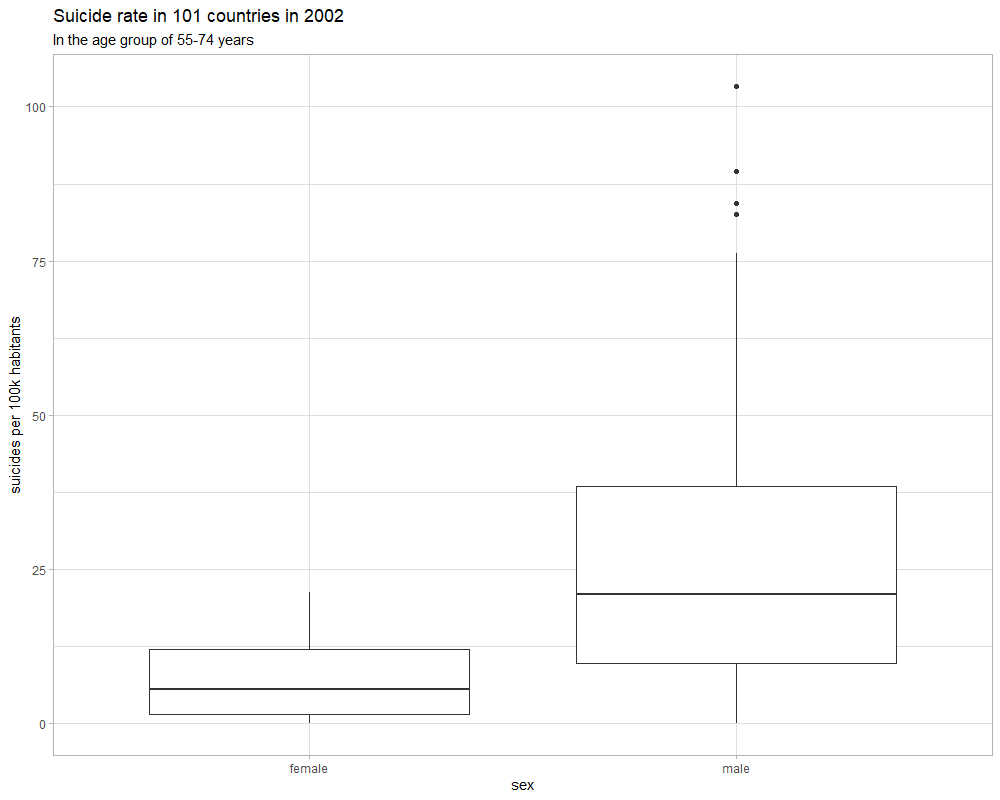
\includegraphics[width=\linewidth]{pergunta_2.png}
\end{center}

\end{document}